\chapter{Non linearities} % (fold)
\label{cha:non_linearities}

\section{Multitone signals} % (fold)
\label{sec:multitone_signals}

Usually we deal with multitone signal as:

\begin{equation}
	V = Acos(\omega_1 t) + Acos(\omega_2t)+Acos(\omega_3t)+...
\end{equation}

Supposing $P_{t_n}$ as the power of one single tone which is proportional to $A^2$ we can define:

\subsection{Average Power} % (fold)
\label{ssub:average_power}

\begin{equation}
	P_a= NkA^2 = NP_t 
\end{equation}

% subsubsection average_power (end)

\subsection{Peak Power} % (fold)
\label{ssub:peak_power}

The peak power in obtained when all the components reach their maximum peak leading to:

\begin{equation}
 	P_p= k (NA)^2= N^2P_t
 \end{equation} 

% subsubsection peak_power (end)

\subsection{Peak Factor} % (fold)
\label{ssub:peak_factor}

\begin{equation}
	F= \frac{P_p}{P_a}
\end{equation}


Note that if every tone has the same amplitude then $F=N$

% subsubsection peak_factor (end)
% section multitone_signals (end)

\section{Effects of distortion. Two-tone test and IIP3.}

When two signals ($\omega_1$, $\omega_2$) at different frequencies are applied to a nonlinear system, the output exhibits components that are not harmonics of these frequencies, but are instead located at characteristic frequencies given by: 
\begin{equation}
	\omega = 2\omega_1 \pm \omega_2
\end{equation}
\begin{equation}
	\omega = 2\omega_2 \pm \omega_1
\end{equation}
These components may corrupt the signal if the latter's frequency matches (or falls within the band of) these components, which are called intermodulation (IM) products. The amplitude of these components is given by: 
\begin{equation}
A_{IM} = \frac{3\alpha_3A_1^2A_2}{4}
\end{equation}
where A$_1$, A$_2$ are the amplitudes of the two interferers and $\alpha_3$ is the third-harmonics coefficient of the modulated output y(t). 
Note that if these amplitudes, and particularly the one of the IM product matching the signal, becomes comparable with the latter, corruption becomes ineliminable even with the use of extremely sharp filters, since it falls in the bandwidth of interest. 
In order to measure intermodulation, a figure of merit is introduced named IIP3 (Input Third Intercept Point), generally measured by means of a "two-tone" test: two pure sinusoids\footnote{A pure sinusoid at a given frequency is generally called "tone".} of equal amplitude are applied to the input, and the amplitude of the IM products at the output is measured together with the amplitude of the fundamental component: 
\begin{equation}
	A_{y,I} = \alpha_1A
\end{equation}
\begin{equation}
	A_{y,IMP} = \frac{3}{4}\alpha_3 A^3
\end{equation}
It can be easily seen that, by plotting the output amplitudes on a log-log scale, the fundamental will show a linear behavior with a +20dB/dec slope, whereas the IM products show the same linear behavior, but with a +60dB/dec slope; the point at which the two lines cross is the IIP3, which can thus be derived by equating the amplitudes of the two measurements: 
\begin{equation}
	A_{y,I}(IIP3) = A_{y,IMP}(IIP3)
\end{equation}
\begin{equation}
	|\alpha_1A_{IIP3}| = |\frac{3}{4}\alpha_3A_{IIP3}^3|
\end{equation}
\begin{equation}
	A_{IIP3} = \sqrt{\frac{4}{3}|\frac{\alpha_1}{\alpha_3}|}
\end{equation}
Note that this is actually an estimation: due to gain compression for higher amplitudes of the input tones, the crossing point between the fundamental's amplitude and the IM3 amplitude at the output shall lie at lower values of A$_{in}$, due to the reduced amplitude of the fundamental component; moreover, higher-order nonlinearities may manifest as A$_{in}$ approaches A$_{IIP3}$, further complicating the picture. An alternative way to measure IIP3, therefore, consists in using an extremely low input level, so that the gain is not compressed and higher order nonlinearities are negligible: by then increasing A$_{in}$ and plotting the resulting amplitudes, we can extrapolate the aforementioned linear plot and determine IIP3 more accurately.
However,  extrapolation can be a long and tedious process, so a shortcut providing a reasonable initial estimate is employed. Considering to have an input equal to A$_{IIP3}$, then the extrapolated output IM products are as ample as the fundamental tone. By reducing the input to a given level A$_{in,1}$, then the change of the input is given by: 
\begin{equation}
	\Delta P = 20\log(A_{IIP3}) - 20\log(A_{in,1})
\end{equation}
Since the output amplitude of the fundamental has a slope of +20dB/dec, whereas the amplitude of the IM3 component has a slope of +60dB/dec, the difference between the two plots has a slope of -40dB/dec. This means that by changing the input amplitude by a quantity $\Delta$P, the difference between the two slopes changes by 2$\Delta$P. We can therefore write: 
\begin{equation}
	\Delta P = 20\log(A_{IIP3}) - 20\log(A_{in,1}) = \frac{1}{2}(20\log(A_f) - 20\log(A_{IM}))
\end{equation}
where A$_f$, A$_{IM}$ are the amplitudes of the fundamental component and of the IM products respectively, when the input signal has amplitude A$_{in,1}$. Therefore it is easy to recover: 
\begin{equation}
	20\log(A_{IIP3}) = \frac{\Delta P}{2} + 20\log(A_{in,1})
\end{equation} 

%%%%%%%%%%%%%%%%%%%%%%%%%%%%%%%%%%%%%%%%%%%%%%%%%%%%%%%%

\section{Peak Envelope Power (PEP)} % (fold)
\label{sub:peak_envelope_power_pep_}

PEP it's the instantaneous power delivered at the peak of the modulated signal:


\begin{figure}[h]
	\centering
	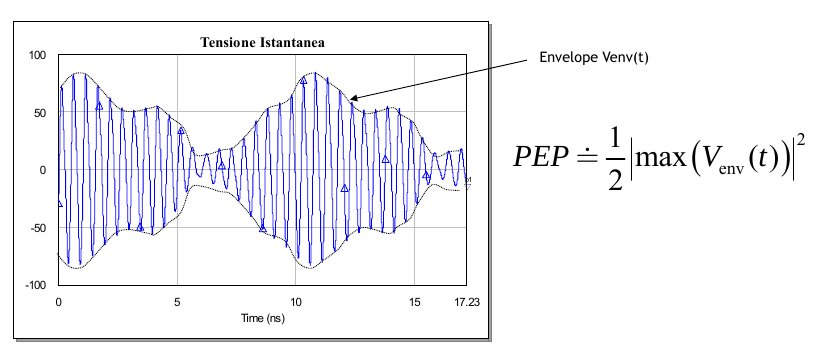
\includegraphics[scale=0.5]{Immagini/pep}
	
	\label{fig:link}
\end{figure}

% subsection peak_envelope_power_pep_ (end)

\section{1dB Compression Point} % (fold)
\label{sec:1db_compression_point}

Given a Polinomial model of an non linear memoryless system:

\begin{equation}
	v_o=a_0+a_1v_i+a_2v_i^2+a_3v_i^3+...
\end{equation}

and cosidering a 1-tone excitation $v_i=Acos(\omega_t) $ we get at the output:

\begin{equation}
	v_o=b_0+b_1cos(\omega_t) +b_2cos(2\omega_t) +b_3cos(3\omega_t) +...
\end{equation}

with:

\begin{itemize}
	\item $b_0= \frac{1}{2}a_2A^2$

	\item $b_1= a_1A+\frac{3}{4}a_3A^3$

	\item $b_2= \frac{1}{2}a_2A^2$

	\item $b_3= \frac{1}{4}a_3A^3$
\end{itemize}

where $b_1$ rappresents the output of the signal at $\omega$ and we can notice that a non linear term is present $\frac{3}{4}a_3A^3$.
In case of amplifiers $a_3$ is usually negative this means that as we increase the input signal amplitude as the non linear negative increase in respect to the linear term thus giving gain compression.

\begin{figure}[h]
	\centering
	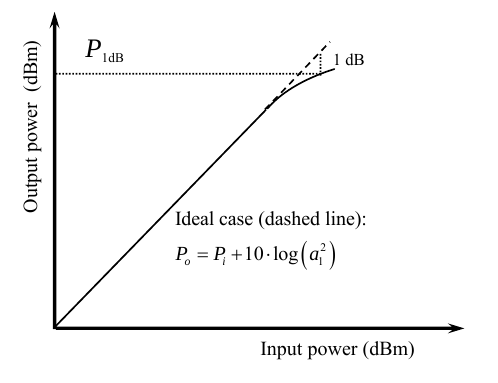
\includegraphics[scale=0.5]{Immagini/1db}
	\caption{Graphical rappresentation of 1dB compression point}
	\label{fig:1db}
\end{figure}


At $P_{1dB}$ the output power is reduced of 1 dB with respect to the one given by the linear term:

\begin{equation}
	P_{1dB}= 10log_{10}\left( \frac{a_1^3}{|a_3|} \right)+0.62dBm
\end{equation}


% section 1db_compression_point (end)

\section{Third order Intercept Point} % (fold)
\label{sec:third_order_intercept_point}

\begin{figure}[h]
	\centering
	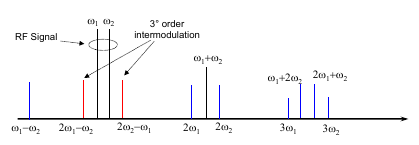
\includegraphics[scale=0.8]{Immagini/spec}
	\caption{Third order intermodulation products in output spectrum}
	\label{fig:spec}
\end{figure}

In Figure~\label{fig:spec} is rappresented a two-tone test and it's output highlighting the intermodulation product.
A two-tone signal is the simplest rappresentation of an RF signal with a certain bandwidth.

We note as the intermodulation products at $(2\omega_1-\omega_2)$ and $(2\omega_2-\omega_1)$ are very close to the signal and considering for example phase noise of the LO it's clear that they can bring to SNR degradation.

\begin{figure}[h]
	\centering
	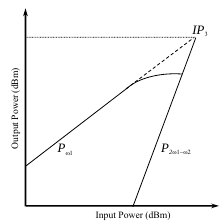
\includegraphics[scale=0.8]{Immagini/ip3}
	\caption{Third order intercept point graphical rappresentation}
	\label{fig:ip3}
\end{figure}


From Figure~\label{fig:ip3} we can derive:

\begin{equation}
	P_{\omega_1}= 10log\left(\left( \frac{a_1A+(9/4)a_3A^3}{\sqrt{2}}\right)^2\frac{1000}{R}\right) \approx 10log\left(\left( \frac{a_1A}{\sqrt{2}}\right)^2\frac{1000}{R}\right)
\end{equation}

\begin{equation}
	P_{2\omega_1-\omega_2}= 10log\left(\left( \frac{(3/4)a_3A^3}{\sqrt{2}}\right)^2\frac{1000}{R}\right)
\end{equation}

from which we can find $IP_3$:

\begin{equation}
	IP_3= 10log\left(\left( \frac{2}{3} \frac{a_1^3}{|a_3|}\right)\frac{1000}{R}\right)
\end{equation}

\begin{equation}
	IP_3 = 10log\frac{a_1^3}{|a_3|}+11.25dBm   \ \ \ \ \ \ (R= 50\Omega)
\end{equation}


\subsection{$P_{1dB}$ and $IP_3$ Relationship} % (fold)
\label{sub:_p_1dB_and_ip_3_relationship}

From $IP_3$ and $P_{1dB}$ definition:

\[
\begin{cases}
	IP_3 = 10log_{10}\left(\frac{a_1^3}{|a_3|}\right) + 11.25dBm\\
	\\
	P_{1dB}= 10log_{10}\left(\frac{a_1^3}{|a_3|}\right) +0.62dBm
\end{cases}
\]

we get:

\begin{equation}
	IP_3= P_{1dB} + \Delta_p \ \ \ \ \ (\Delta_p = 10.63dB)
\end{equation}
% subsection _p_1db_and_ip_3_relationship (end)

\subsection{Mean Power} % (fold)
\label{sub:mean_power}

$Pm =(P_{\omega_1}+3)$

% subsection mean_power (end)


\subsection{Carrier to Intermodulation ratio (CI)} % (fold)
\label{sub:ci_carrier_to_intermodulation_ratio}




\begin{figure}[ht]
	\centering
	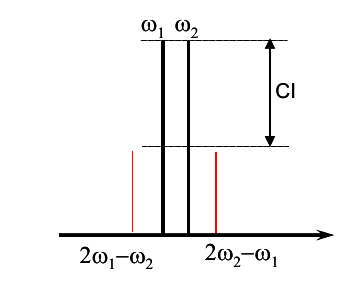
\includegraphics[scale=0.4]{Immagini/ci}
	\label{fig:ci}
\end{figure}
\begin{equation}
	CI_{|dB} \approx 2IP_3 - 2P_m +6= 2(IP_3-P_0) \ \ \ \ \ considering P_{\omega_1} \ll IP_3
\end{equation}

 $Pm =(P_{\omega_1}+3)$ the average power of the two-tone signal.
% subsection ci_carrier_to_intermodulation_ratio (end)


\section{Power amplifiers} % (fold)
\label{sec:power_amplifiers}


\subsection{Output Power and non linearities} % (fold)
\label{sub:output_power_and_non_linearities}

When assigning the output power of a PA, also the corresponding level of
nonlinear distortion it must be specified.
The 2-tone signal is often using as reference excitation. In this case it is
usual to specify the maximum PEP power for which the CI is equal to 30dB:


\begin{equation}
	PEP = P_m +3  \ \ \ \ \ (2 \ tones) 
	\end{equation}
\begin{equation}
	30= 2IP_3-2(PEP-3)+6 \ \ \ \Longrightarrow \ \ \ PEP= IP_3-9 
\end{equation}

from $IP_3=P_{1dB}+\Delta_p$ we get:

\begin{equation}
	PEP= P_{1dB} + (\Delta_p -9 )   \ \ \ \ \ (for \  CI=30dB)
\end{equation}
% subsection output_power_and_non_linearities (end)


\subsection{Back-Off} % (fold)
\label{sub:back_off}

The backoff of a PA is the difference in dB between the output power at $P_{1dB}$ and the average output power. From the previous equations, it can be obtained:

\begin{equation}
	BO\approx \frac{CI_{|dB}}{2}-\Delta_p-3 \ \ \ \ \ (2  \ tones)
\end{equation}


\subsection{Power Added Efficiency (PAE)} % (fold)
\label{sub:power_added_efficiency}


PAE in an important FoM for the ability of a PA to convert DC power to RF power:

\begin{equation}
	PAE= 100\frac{(RF \ Power \ at \ Load)- (RF \ Power \ at \ Input)}{DC \ power}\%
\end{equation}

In the design process we must take into account that to increase linearity PAE should be decreased.
% subsection power_added_efficiency (end)
% subsection back_off (end)

\subsection{Dynamic Range} % (fold)
\label{sub:dynamic_range}

It quantifies the range of power allowed at the receiver input.
The minimum power is defined by the sensitivity S.
The maximum power is conventionally assumed as the mean power of a 2-tone signal producing a IM3 power (referred to the input) equal to the receiver sensitivity (S):
\begin{equation}
DR_{dB}= \frac{2}{3}(IIP_3+3-S_{dBm})	
\end{equation}

where:

\begin{equation}
	IIP_3=\frac{IP_3}{G_{tot}} Input \ Referred \ 3^{rd} order Intercept Point
\end{equation}
% subsection dinamic_range (end)

\section{Cascaded Stages} % (fold)
\label{sec:cascaded_stages}

\begin{figure}[ht]
	\centering
	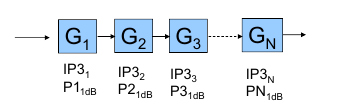
\includegraphics[scale=0.8]{Immagini/casip}
	\caption{Example of a cascaded stage with third order non linearities.}
	\label{fig:casip}
\end{figure}

% section cascaded_stages (end)
\subsection{Cascaded Stage IIP3} % (fold)
\label{sec:cascaded_stage_iip3}


\begin{equation}
\left ( \frac {1} {IIP3} \right)^2 = \left( \frac {1} {IIP3_1}  \right)^2 + \left( \frac{G_1}{IIP3_2}  \right)^2 + \left( \frac {G_1G_2} {IIP3_3}  \right)^2 + ...\left( \frac {G_1G_2...G_{n-1}} {IIP3_n}  \right)^2
\end{equation}

\subsection{Cascaded 1dB Compression Point}
\begin{equation}
\left ( \frac {1} {P_{1dB}} \right)^2 = \left( \frac {1} {P_{1_{1dB}}}  \right)^2 + \left( \frac{G_1}{P_{2_{1dB}}}  \right)^2 + \left( \frac {G_1G_2} {P_{3_{1dB}}}  \right)^2 + ...\left( \frac {G_1G_2...G_{n-1}} {P_{N_{1dB}}}  \right)^2
\end{equation}


% section third_order_intercept_point (end)


% chapter non_linearities (end)